% ===========================================================================
% Part VIII - Probabilistic Sequence Modeling: Hidden Markov Models (Experiment 16)
% ===========================================================================

\part{Probabilistic Sequence Modeling: Hidden Markov Models}

% ---------------------------------------------------------------------------
\chapter{Hidden Markov Model (HMM)}\label{exp:16}

\runninghead{Experiment 16: Hidden Markov Model (HMM)}

\quickfacts
  {Dataset}{DAX stock index 1991--1998 (\texttt{data/stock\_index.csv}, real \texttt{EuStockMarkets}); 1,859 trading days}
  {Key parameters}{3 Gaussian states, full covariance, 200 Baum--Welch (EM) iterations; Viterbi decoding}
  {Headline result}{EM converged; log-likelihood 6019.79; volatility-sorted Bull / Sideways / Bear regimes}

\section{Objective}
Model a sequence using hidden states, transition probabilities and emission distributions;
decode the most likely hidden-state path with the Viterbi algorithm.

\section{Suggested Dataset}
Real DAX stock index daily closes 1991--1998 (\texttt{data/stock\_index.csv}, R
\texttt{EuStockMarkets}), 1,859 trading days. The observation sequence is the daily return;
the close price is used only for plotting.

\section{Required Libraries}
hmmlearn, numpy, pandas, matplotlib.

\section{Brief Theory}
A Hidden Markov Model is a doubly stochastic process:
\begin{itemize}
  \item a hidden state sequence $z_t$ following a first-order Markov chain,
        $P(z_t \mid z_{t-1}, \dots, z_1) = P(z_t \mid z_{t-1})$, summarized by the transition
        matrix $A_{ij} = P(z_{t+1} = s_j \mid z_t = s_i)$;
  \item observations emitted from the active state,
        $x_t \mid (z_t = s_k) \sim \mathcal{N}(\mu_k, \sigma_k^2)$ for a Gaussian HMM.
\end{itemize}
Three classical problems are solved here: \textbf{evaluation} (the forward algorithm gives
$P(X \mid \lambda)$), \textbf{decoding} (the Viterbi algorithm finds the most likely state
path by dynamic programming) and \textbf{learning} (Baum--Welch EM alternates a
forward--backward E-step with parameter re-estimation until the log-likelihood converges).

\section{Procedure}
\begin{enumerate}
  \item Load the DAX series and build the daily-return observation vector.
  \item Fit a 3-state Gaussian HMM with full covariance and 200 EM iterations.
  \item Check convergence and the model log-likelihood.
  \item Decode the state path with Viterbi.
  \item Sort the states by volatility so they map to Bull/Sideways/Bear; reorder the transition
        matrix accordingly.
  \item Plot the transition heatmap and the price series colored by regime.
\end{enumerate}

\section{Reference Implementation}
\begin{codebox}[title={Fitting, decoding and volatility-sorting the HMM}]
hmm_model = GaussianHMM(n_components=3, covariance_type="full", n_iter=200, random_state=42)
hmm_model.fit(returns)
hidden_states = hmm_model.predict(returns)                 # Viterbi
state_order = np.argsort([np.sqrt(hmm_model.covars_[i][0][0]) for i in range(3)])
\end{codebox}

\section{Evaluation / Expected Output}
\begin{table}[htbp]
  \centering
  \caption{Gaussian HMM on the DAX index (1,859 trading days, 1991--1998).}
  \begin{tabular}{|l|r|}
    \hline
\rowcolor{mlblue!8}    \textbf{Item} & \textbf{Value} \\
    \hline
    EM converged & True \\
\hline
    Model log-likelihood & \best{6019.79} \\
\hline
    Regimes & Bull (low vol), Sideways (medium), Bear (high vol) \\
    \hline
  \end{tabular}
\end{table}

\begin{figure}[htbp]
  \centering
  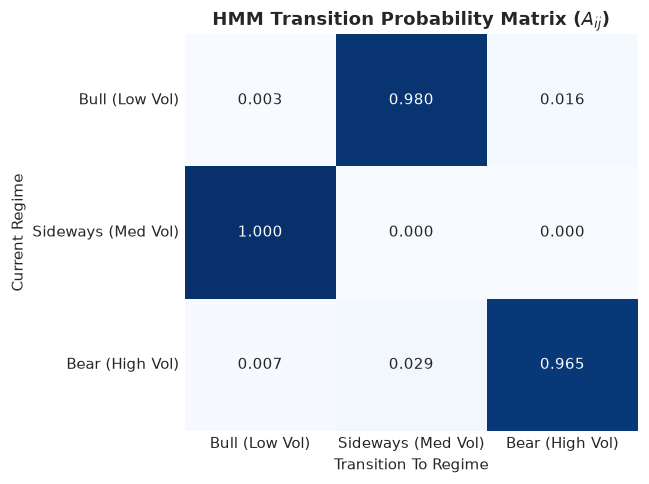
\includegraphics[width=0.60\textwidth]{figures/exp16_transition_matrix.png}
  \caption{Estimated transition-probability matrix after sorting the states by volatility;
  the dominant diagonal indicates regime persistence.}
  \label{fig:exp16-trans}
\end{figure}

\begin{figure}[htbp]
  \centering
  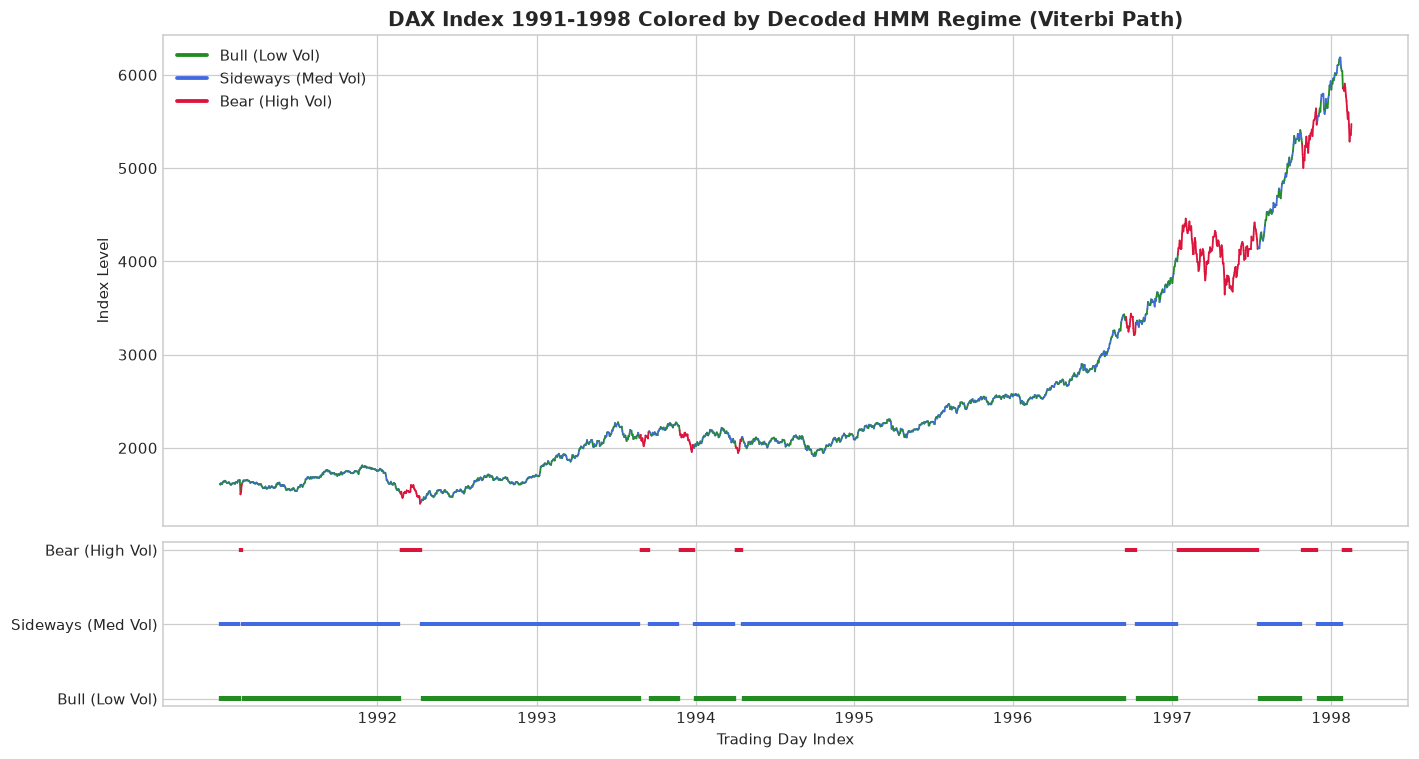
\includegraphics[width=0.95\textwidth]{figures/exp16_dax_regimes.png}
  \caption{DAX index 1991--1998 colored by the Viterbi-decoded regime (top) and the decoded
  state sequence over time (bottom).}
  \label{fig:exp16-dax}
\end{figure}

The model extracts interpretable, persistent market regimes from real data without labels. The
colored DAX chart tracks real episodes: the 1990s bull phases, corrections such as 1994, and
the high-volatility cluster around the 1998 crisis. Its main assumptions are the Markov
property and Gaussian emissions; return fat tails and duration dependence motivate extensions
such as $t$-emissions or semi-Markov models.

\section{Viva / Discussion Questions}
\begin{description}
  \item[What is hidden in an HMM?] The state sequence: we observe emissions (returns) but not
  the underlying regime that generated them.
  \item[Viterbi vs forward algorithm?] Viterbi returns the single most likely state path (a
  maximum over paths); the forward algorithm computes the total probability $P(X \mid \lambda)$
  by summing over all paths.
  \item[What is the Markov assumption?] The future state depends on the past only through the
  present state: $P(z_t \mid z_{1:t-1}) = P(z_t \mid z_{t-1})$.
  \item[Why sort the states by volatility?] So that regime labels (Bull/Sideways/Bear) are
  stable and interpretable across runs.
  \item[Why model returns and not prices?] Returns are approximately stationary; prices trend
  and violate the Gaussian emission assumption.
\end{description}

\FloatBarrier
\section{Complete Code Listing}
% ===========================================================================
% exp16_hmm.tex - complete code listings for Experiment 16
% Source: notebooks/08_hidden_markov_model.ipynb (executed)
% ===========================================================================

\begin{codebox}[title={Core libraries}]
# ---- Core libraries ----
import numpy as np
import pandas as pd
import matplotlib.pyplot as plt
import seaborn as sns
from hmmlearn.hmm import GaussianHMM

# Styling setup
plt.style.use('seaborn-v0_8-whitegrid' if 'seaborn-v0_8-whitegrid' in plt.style.available else 'default')
plt.rcParams['font.sans-serif'] = 'DejaVu Sans'
plt.rcParams['figure.figsize'] = (10, 6)
plt.rcParams['figure.dpi'] = 110
np.random.seed(42)

# ---- Load the real DAX stock index (daily closes 1991-1998) ----
df_market = pd.read_csv('../data/stock_index.csv')
dates = pd.to_datetime(df_market['Date'])
print(f"Trading days: {len(df_market)} | {dates.iloc[0].date()} to {dates.iloc[-1].date()}")
print(df_market.head(3).to_string(index=False))

returns = df_market['Daily_Return'].values.reshape(-1, 1)   # HMM observations
prices = df_market['Close'].values                          # only used for visualization
\end{codebox}

\begin{codebox}[title={Fit a 3-state Gaussian HMM with the Baum-Welch (EM) algorithm}]
# ---- Fit a 3-state Gaussian HMM with the Baum-Welch (EM) algorithm ----
n_components = 3
hmm_model = GaussianHMM(
    n_components=n_components,        # Bull / Sideways / Bear regimes
    covariance_type="full",           # each state has its own full covariance Gaussian emission
    n_iter=200,                       # EM iterations
    random_state=42,
    verbose=False
)

hmm_model.fit(returns)
print("EM Training Converged:", hmm_model.monitor_.converged)
print(f"Model Log-Likelihood: {hmm_model.score(returns):.2f}")

# ---- Decode the most likely hidden state sequence with the Viterbi algorithm ----
hidden_states = hmm_model.predict(returns)

# ---- Sort regimes by volatility so labels have a consistent economic meaning ----
# Regime 0: Low Volatility (Bull) | Regime 1: Moderate (Sideways) | Regime 2: High (Bear/Crisis)
volatilities = [np.sqrt(hmm_model.covars_[i][0][0]) for i in range(n_components)]
state_order = np.argsort(volatilities)                                           # ascending volatility
state_mapping = {old_state: new_state for new_state, old_state in enumerate(state_order)}

sorted_hidden_states = np.array([state_mapping[s] for s in hidden_states])       # relabel sequence
sorted_means = [hmm_model.means_[old][0] for old in state_order]                 # reordered means
sorted_stds  = [np.sqrt(hmm_model.covars_[old][0][0]) for old in state_order]    # reordered std devs

# ---- Reorder the transition matrix to match the sorted regimes ----
sorted_transmat = np.zeros((n_components, n_components))
for i in range(n_components):
    for j in range(n_components):
        sorted_transmat[i, j] = hmm_model.transmat_[state_order[i], state_order[j]]

regime_names = ["Bull (Low Vol)", "Sideways (Med Vol)", "Bear (High Vol)"]
\end{codebox}

\begin{codebox}[title={Transition probability matrix}]
# ---- Transition probability matrix ----
fig, ax = plt.subplots(figsize=(6, 4.5))
sns.heatmap(sorted_transmat, annot=True, fmt='.3f', cmap='Blues', ax=ax,
            xticklabels=regime_names, yticklabels=regime_names, cbar=False)
ax.set_title("HMM Transition Probability Matrix ($A_{ij}$)", fontweight='bold')
ax.set_xlabel("Transition To Regime")
ax.set_ylabel("Current Regime")
plt.tight_layout()
plt.show()

# ---- Viterbi-decoded regimes over the price series ----
colors = ['forestgreen', 'royalblue', 'crimson']
x = np.arange(len(prices))

fig, (ax1, ax2) = plt.subplots(2, 1, figsize=(13, 7), sharex=True, gridspec_kw={'height_ratios': [3, 1]})

# Top: color every consecutive price segment by its decoded regime
for i in range(len(prices) - 1):
    ax1.plot([x[i], x[i + 1]], [prices[i], prices[i + 1]], color=colors[sorted_hidden_states[i]], lw=1.2)
for i, name in enumerate(regime_names):
    ax1.plot([], [], color=colors[i], label=name, lw=2.5)
ax1.set_title("DAX Index 1991-1998 Colored by Decoded HMM Regime (Viterbi Path)", fontsize=13, fontweight='bold')
ax1.set_ylabel("Index Level")
ax1.legend(loc='upper left')

# Bottom: raw sequence of decoded states over time
ax2.scatter(x, sorted_hidden_states, c=[colors[s] for s in sorted_hidden_states], s=8, marker='|')
ax2.set_yticks(range(n_components))
ax2.set_yticklabels(regime_names)
ax2.set_xlabel("Trading Day Index")

# Label the x-axis with years (real dates)
year_pos = np.where(dates.dt.year.diff().fillna(0).values != 0)[0]
ax2.set_xticks(year_pos)
ax2.set_xticklabels(dates.dt.year.iloc[year_pos].astype(str))

plt.tight_layout()
plt.show()
\end{codebox}

